\documentclass[14pt]{extreport}
\usepackage{caption}
\usepackage[utf8]{inputenc}
\usepackage[T2A]{fontenc}
\usepackage[english,ukrainian]{babel}
\usepackage{tempora}
\usepackage{float}
\linespread{1.5}
\usepackage{longtable}
\setlength{\parskip}{0pt}
\usepackage{indentfirst}
\usepackage{graphicx}
\usepackage{cmap}
\usepackage{longtable}
\usepackage{titlesec}
\usepackage{geometry}
\usepackage{listings}
\renewcommand{\arraystretch}{1.5}
\geometry{
	a4paper,
	left=20mm,
	right=20mm,
	top=15mm,
	bottom=15mm,
}

\graphicspath{ {./pictures} }
\setlength{\parindent}{4em}

\newcommand\subject{Людино-машинна взаємодія (вбудовані системи)}
\newcommand\lecturer{доцент кафедри ПЗ\\Федорчук Є.Н.}
\newcommand\teacher{доцент кафедри ПЗ\\Федорчук Є.Н.}
\newcommand\mygroup{ПЗ-42}
\newcommand\lab{2}
\newcommand\theme{Моделювання людино-машинної взаємодії (ЛМВ) у ВС
для моніторингу надзвичайної ситуації}
\newcommand\purpose{Навчитися моделювати людино-машинну взаємодію у
вбудованих системах}

\begin{document}
\begin{normalsize}
	\begin{titlepage}
		\thispagestyle{empty}
		\begin{center}
			\textbf{МІНІСТЕРСТВО ОСВІТИ І НАУКИ УКРАЇНИ\\
				НАЦІОНАЛЬНИЙ УНІВЕРСИТЕТ "ЛЬВІВСЬКА ПОЛІТЕХНІКА"}
		\end{center}
		\begin{flushright}
			\textbf{ІКНІ}\\
			Кафедра \textbf{ПЗ}
		\end{flushright}
		\vspace{20pt}
		\begin{center}
			\textbf{ЗВІТ}\\
			\vspace{10pt}
			до лабораторної роботи № \lab\\
			\textbf{на тему}: <<\textit{\theme}>>\\
			\textbf{з дисципліни}: <<\subject>>
		\end{center}
		\vspace{20pt}
		\begin{flushright}
			
			\textbf{Лектор}:\\
			\lecturer\\
			\vspace{28pt}
			\textbf{Виконав}:\\
			
			студенти групи \mygroup\\
			Коваленко Д.М.\\
			\vspace{28pt}
			\textbf{Прийняв}:\\
			
			\teacher\\
			
			\vspace{28pt}
			«\rule{1cm}{0.15mm}» \rule{1.5cm}{0.15mm} 2025 р.\\
			$\sum$ = \rule{1cm}{0.15mm}……………\\
			
		\end{flushright}
		\vspace{\fill}
		\begin{center}
			\textbf{Львів — 2025}
		\end{center}
	\end{titlepage}
		
	\begin{description}
		\item[Тема.] \theme.
		\item[Мета.] \purpose.
	\end{description}

  \section*{Лабораторне завдання}
  \begin{enumerate}
  	\item Проектувати архітектуру ПЗ з врахуванням функціональних вимог.
  \item Обрати формат діалогу у вигляді сценаріїв-послідовне відображення
кадрів кожного вікна.
  \item Розробити шаблони кадрів (уведення даних, виведення повідомлень,
виведення тривожних повідомлень).
  \item Для кожного шаблону описати необхідну множину процедур
виведення повідомлень.
  \item Описати множину процедур уведення даних.
  \item Обрати для шаблонів ергономічні часові межі опрацювання інформації.
  \item Оформити звіт у формі таблиці. Стовбці – назви завдань за пунктами списку. Для окремих завдань може бути декілька стовбців.Рядки – чисельно-символьний опис реалізації завдань.
  \item Розробити ПЗ для реалізації діалогу ЛМВ за допомогою багатовіконного інтерфейсу.
  \item Виконати тестування ПЗ.
  \item Оформити звіт з використанням візуальних форм ЛМВ.
  \end{enumerate}
  
  \section*{Хід роботи}
  
   % Add this to the preamble

  \renewcommand{\tablename}{Таблиця}
  \renewcommand{\thetable}{\arabic{table}}
  \captionsetup{justification=raggedleft, singlelinecheck=false, labelsep=period}

\begin{longtable}{|l|p{4cm}|p{4cm}|p{3cm}|p{3cm}|}
\caption{Результати проектування інтерфейсу} \\
\hline
\textbf{№} & \textbf{Формат діалогу} & \textbf{Шаблон кадру} & \textbf{Множина процедур введення даних} & \textbf{Ергономічні часові межі} \\ \hline
\endfirsthead
\multicolumn{5}{c}%
{} \\
\hline
\textbf{№} & \textbf{Формат діалогу} & \textbf{Шаблон кадру} & \textbf{Множина процедур введення даних} & \textbf{Ергономічні часові межі} \\ \hline
\endhead
\endfoot
\hline
\endlastfoot
\textbf{1} & Викликає вікна
№2 та №3,
отримує дані
від вікна №2
для
відображення. & Чотири
ділянки, що являють собою
представлення параметрів
надзвичайної ситуації
(рівень води, температура,
сніг, дощ). & \textbf{$V = \{V_t, V_i\}$} & 0,1 \\ \hline
\textbf{2} & Отримує
початковийсписок даних
від вікна №1.
Отримує
інформацію
про появу чи
відбій загроз
від
користувача & Вікно містить в собі форму,
в якій обирається параметрнадзвичайної ситуації. & \textbf{$V = \{V_t, V_i\}$} & 0,1 \\ \hline
\textbf{3} & Викликається
вікном №1,
якщо було
змінено стан
одного з
параметрів
надзвичайної
ситуації. & Вікно-повідомлення.
Містить в собі:
повідомлення про дії для
населення; картинку, що
відповідає певному рівню
загрози. &  \textbf{$V = \{V_t, V_i, V_a\}$} & 0,1 \\ \hline
\end{longtable}
	
	\begin{figure}[H]
	  \centering
	  \includegraphics[scale=0.7]{1}
	  \caption{Вікно моніторингу появи та відбою загроз (вікно №1)}
	\end{figure}
	
	\begin{figure}[H]
	  \centering
	  \includegraphics[scale=0.8]{2}
	  \caption{Вікно повідомлення про появу та відбій загроз (вікно №2)}
	\end{figure}
	
	\begin{figure}[H]
	  \centering
	  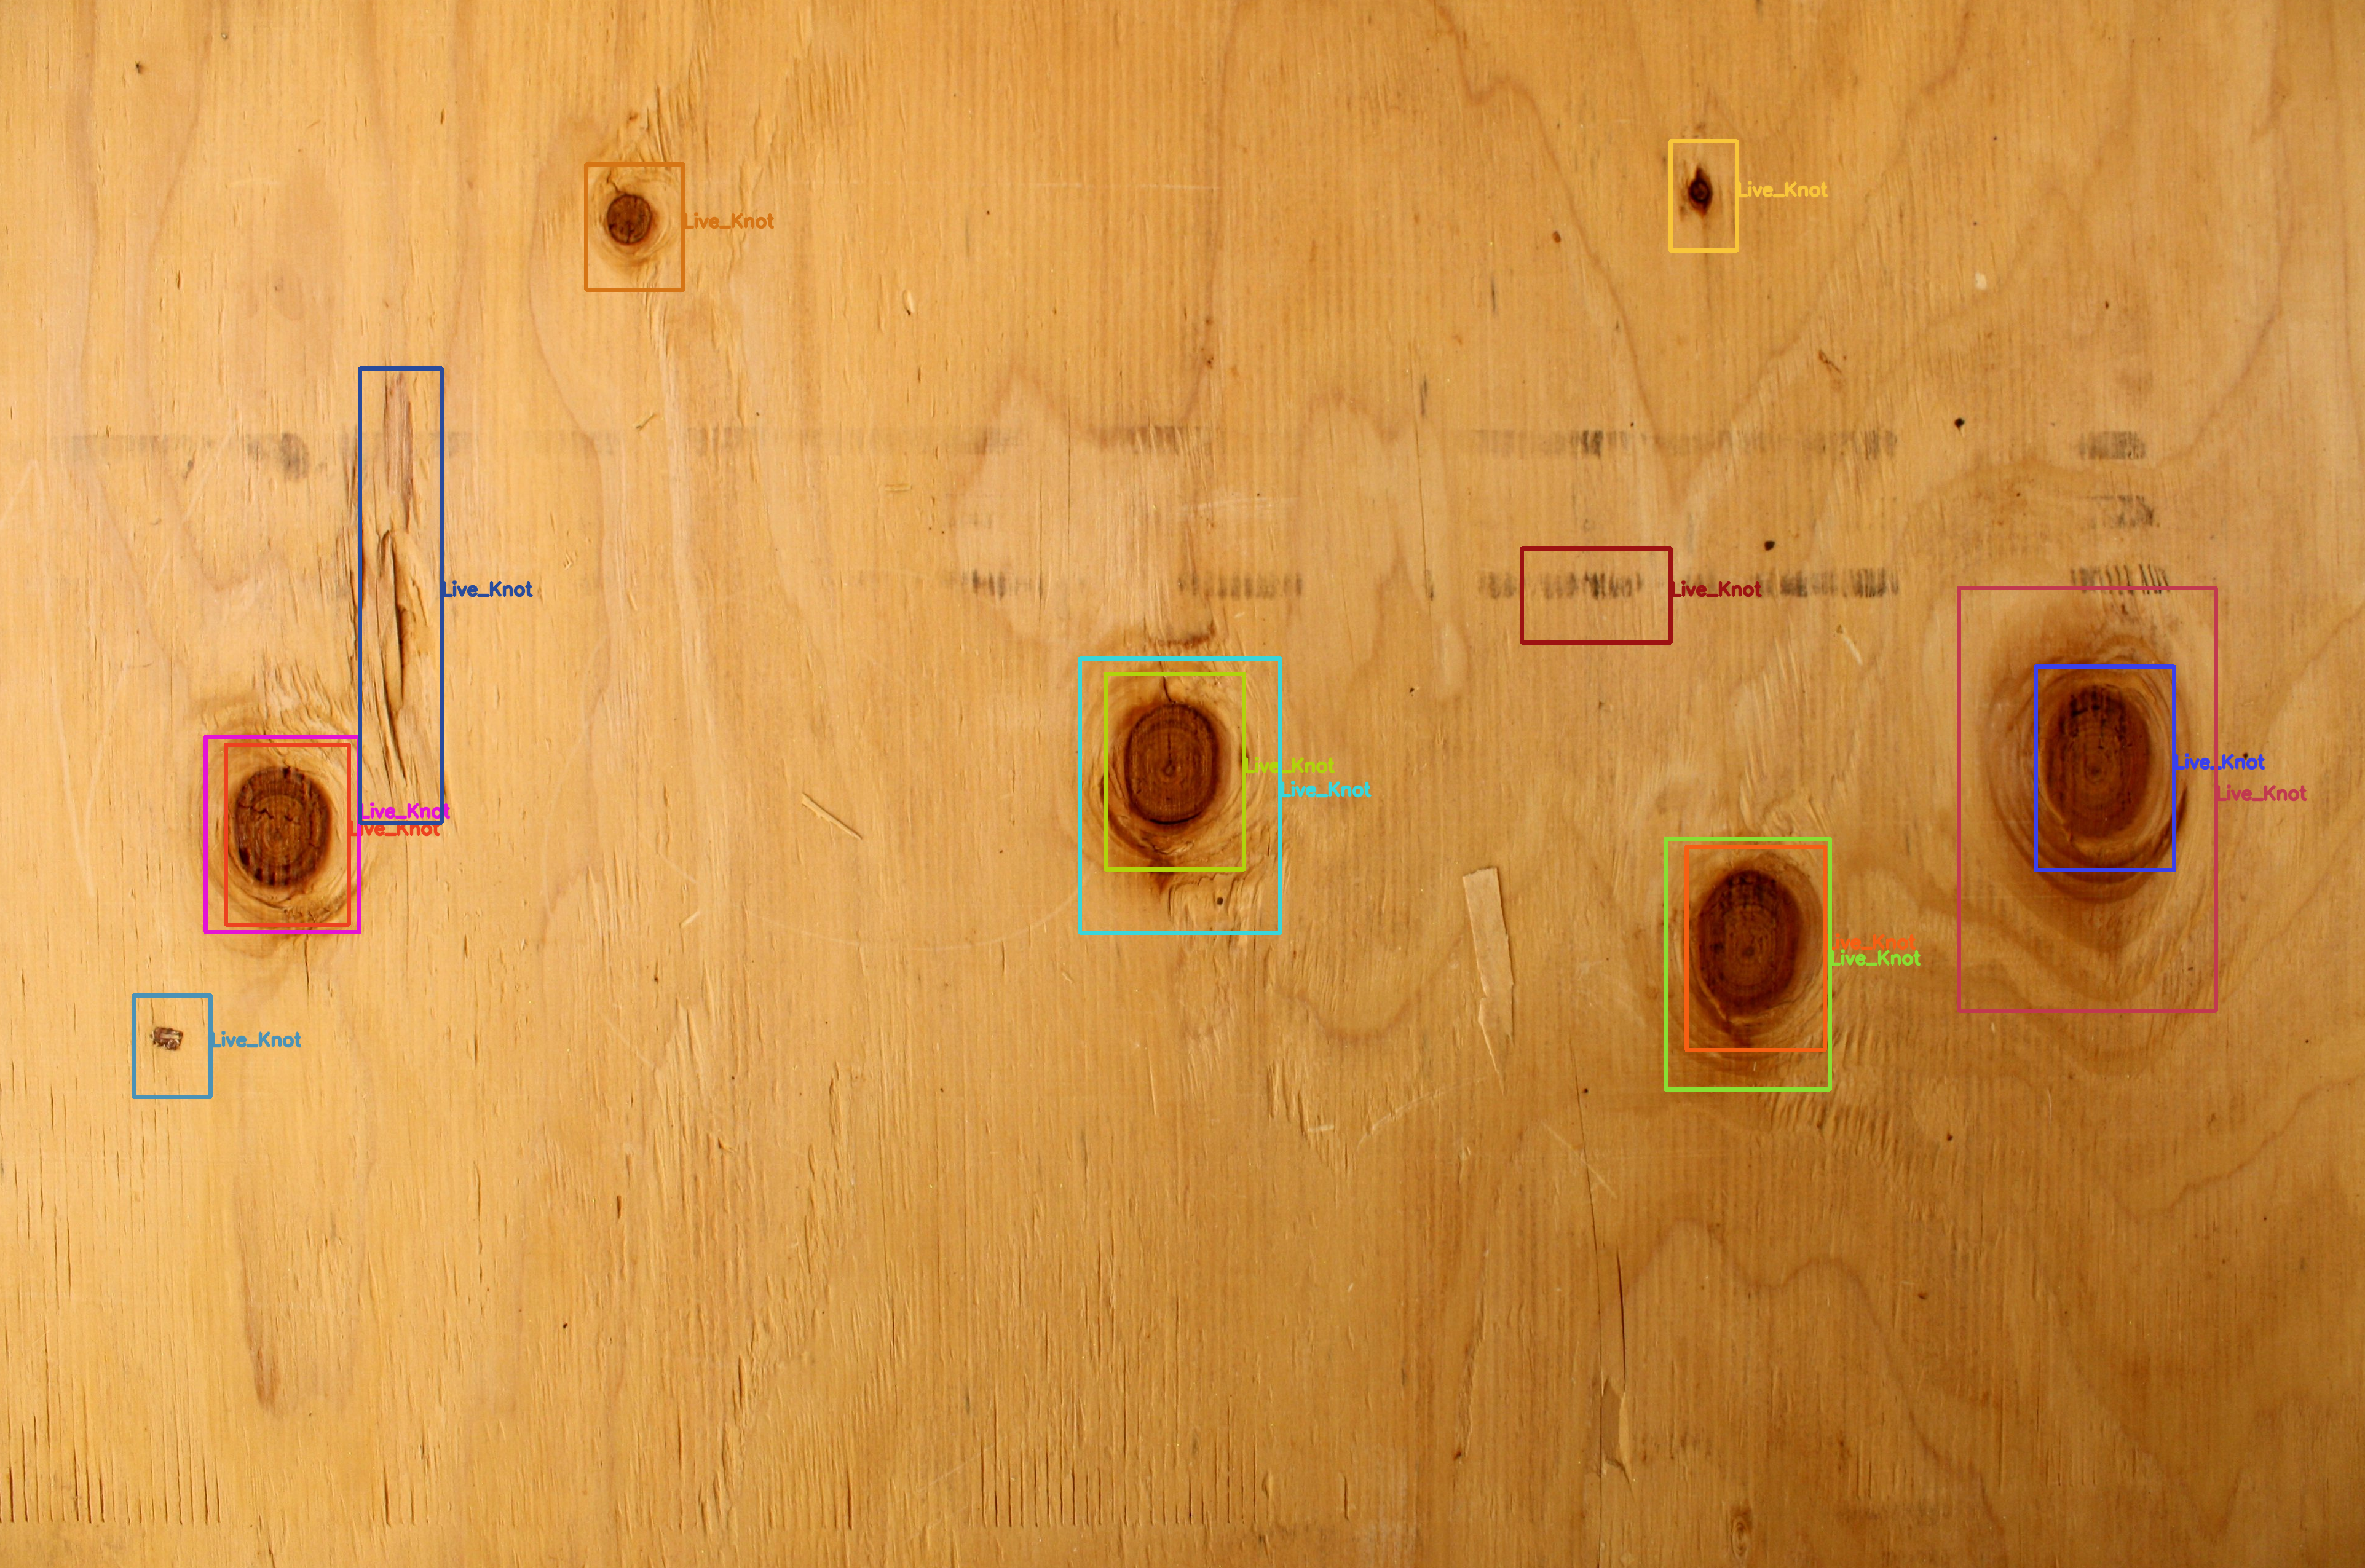
\includegraphics[scale=0.8]{3}
	  \caption{Вікно оповіщення про появу та відбій загроз (вікно №3)}
	\end{figure}
	
	\section*{Висновки}
	
	Під час даної лабораторної роботи навчився проектувати інтерфейс з використанням характеристик людино-машинної взаємодії. Визначив скільки вікон матиме багатовіконний інтерфейс, формат діалогу вікон, їх шаблони, множини процеду введення даних, ергономічні часові межі опрацювання інформації. Створив діаграми прецедентів та класів розроблюваної системи, завдяки ним реалізовував проект. Під час процесу тестування знайшов та виправив помилки системи.
	
	    
\end{normalsize}
\end{document}
